\chapter{Dispersión y paquetes de ondas}\label{ch:b2:dispersion-wave-packets}

Tírese una piedra a un estanque y obsérvese el anillo de ondas: nacen
crestas nuevas en su borde interior, lo recorren hacia fuera y mueren en
su borde exterior --- el anillo entero se mueve más despacio que las
crestas que lo forman. Siéntese uno en una playa después de una tormenta
lejana y el mar de fondo, largo y lento, llegará un día antes que el
oleaje corto: el mar clasifica las ondas por su longitud de onda. El
primer cable telegráfico transatlántico, en 1858, convertía puntos y rayas
nítidos en un borrón que costaba minutos leer. En los tres casos la
celeridad de una onda depende de su frecuencia: el medio es
\emph{dispersivo}. Este capítulo presenta la \omterm{def:b2:dispersion-wave-packets:relation}{relación de dispersión}, el
\omterm{def:b2:dispersion-wave-packets:complex}{número de onda complejo} que lleva a la vez la propagación y la absorción,
la \omterm{prop:b2:dispersion-wave-packets:group}{velocidad de grupo} a la que viaja realmente un paquete --- y su
energía, y su información --- y la línea por la que han viajado la
telegrafía, la televisión e internet: el \omterm{prop:b2:dispersion-wave-packets:coax}{cable coaxial}.

\section{La relación de dispersión}

\begin{definition}[Relación de dispersión; velocidad de fase]\label{def:b2:dispersion-wave-packets:relation}
\index{relación de dispersión}\index{velocidad de fase}\index{medio dispersivo}
Un medio lineal, homogéneo e invariante en el tiempo admite las ondas
planas monocromáticas $\underline s = A\,\eu^{\iu(\omega t - kx)}$ (en
notación compleja; la señal física es la parte real) siempre que $\omega$ y $k$
cumplan la \emph{relación de dispersión} del medio, $\mathcal D(\omega, k)
= 0$, resuelta como $k(\omega)$ o como $\omega(k)$. Para $k$ real la onda viaja
sin deformarse a la \emph{velocidad de fase}
\[
v_\varphi = \frac\omega k .
\]
El medio es \emph{no dispersivo} cuando $v_\varphi$ no depende de $\omega$
(entonces $\omega = ck$ y toda señal se propaga sin deformarse --- la
\omterm{thm:b2:waves-on-strings:equation}{ecuación de d'Alembert}), y \emph{dispersivo} en caso contrario.
\end{definition}

\begin{proof}
Sustituir $\eu^{\iu(\omega t - kx)}$ en una ecuación lineal de coeficientes
constantes convierte cada $\partial_t$ en $\iu\omega$ y cada $\partial_x$ en
$-\iu k$, y deja una relación algebraica. La cuerda, la onda sonora y la
barra dieron $\omega^2 = c^2k^2$.
\end{proof}

\begin{example}[Medios dispersivos y no dispersivos]\label{ex:b2:dispersion-wave-packets:examples}
\index{ecuación de Klein--Gordon}\index{ondas en aguas profundas}
(i) Una cuerda sobre un lecho elástico (fuerza recuperadora $-Ky$ por
unidad de longitud, o una cadena de péndulos), $\mu\partial_t^2y = T\partial_x^2y - Ky$: $\omega^2 = \omega_c^2
+ c^2k^2$ con $\omega_c = \sqrt{K/\mu}$ --- la relación de
\emph{Klein--Gordon}, la misma que la de un plasma y la de una guía de
ondas (\cref{ch:b2:waves-in-media,ch:b2:guided-waves}): $v_\varphi = c/\sqrt{1 -
\omega_c^2/\omega^2} > c$, y ningún $k$ real por debajo de la \emph{frecuencia de corte} $\omega_c$.
(ii) Ondas de gravedad en aguas profundas: $\omega^2 = gk$ (admitida), $v_\varphi =
\sqrt{g/k} = \sqrt{g\lambda/2\pi}$: las ondas largas son más rápidas --- \qty{12.5}{m/s} para
\qty{100}{m} y \qty{40}{m/s} para \qty{1}{km}. (iii) La \omterm{prop:b2:waves-on-strings:chain}{cadena de átomos}, $\omega =
2\omega_0|\sin(ka/2)|$ (\cref{ch:b2:waves-on-strings}). (iv) La luz en el vidrio,
$k = n(\omega)\omega/c$, y por eso un prisma despliega un espectro.
\end{example}

\begin{omfigure}
\begin{tikzpicture}
\begin{axis}[omaxis, axis x line=bottom, axis y line=left, width=6.2cm, height=4.6cm,
    xlabel={$k$}, ylabel={$\omega$}, xmin=0, xmax=3, ymin=0, ymax=3.3, xtick=\empty, ytick={1}, yticklabels={$\omega_c$}, samples=80,
    xlabel style={at={(axis description cs:1.0,0.0)}, anchor=west},
    ylabel style={at={(axis description cs:0.0,1.0)}, anchor=south},
    legend style={font=\scriptsize, at={(0.03,0.97)}, anchor=north west, draw=none, fill=none}]
  \addplot[omDef, thick, domain=0:3] {x};
  \addplot[omThm, thick, domain=0:3] {sqrt(1+x*x)};
  \addplot[omProp, thick, domain=0:3] {1.6*sqrt(x)};
  \legend{$\omega = ck$, $\omega^2 = \omega_c^2 + c^2k^2$, $\omega^2 = gk$}
\end{axis}
\end{tikzpicture}
\hfill
\begin{tikzpicture}
\begin{axis}[omaxis, axis x line=bottom, axis y line=left, width=6.2cm, height=4.6cm,
    xlabel={$\omega/\omega_c$}, ylabel={$v/c$}, xmin=0, xmax=4, ymin=0, ymax=2.6, xtick={1,2,3}, ytick={1}, samples=100,
    xlabel style={at={(axis description cs:0.5,-0.12)}, anchor=north},
    ylabel style={at={(axis description cs:-0.1,0.5)}, rotate=90, anchor=south},
    legend style={font=\scriptsize, at={(0.97,0.95)}, anchor=north east, draw=none, fill=none}]
  \addplot[omThm, thick, domain=1.08:4] {1/sqrt(1-1/(x*x))};
  \addplot[omDef, thick, domain=1.0:4] {sqrt(1-1/(x*x))};
  \addplot[black, dashed, domain=0:4] {1};
  \legend{$v_\varphi$, $v_g$}
  \node[font=\scriptsize, anchor=west, align=left] at (axis cs:0.05,1.9) {sin\\propagación};
\end{axis}
\end{tikzpicture}

{\small A la izquierda, tres relaciones de dispersión: una recta para un
medio no dispersivo, la hipérbola de Klein--Gordon con su frecuencia de
corte y la parábola de las \omterm{ex:b2:dispersion-wave-packets:examples}{ondas en aguas profundas}. A la derecha, para la
relación de Klein--Gordon la \omterm{def:b2:dispersion-wave-packets:relation}{velocidad de fase} supera a $c$ y la \omterm{prop:b2:dispersion-wave-packets:group}{velocidad
de grupo} se queda por debajo, con $v_\varphi v_g = c^2$.}
\end{omfigure}

\begin{definition}[Número de onda complejo: propagación y atenuación]\label{def:b2:dispersion-wave-packets:complex}
\index{número de onda complejo}\index{atenuación}\index{onda evanescente}\index{profundidad de penetración}
Cuando la \omterm{def:b2:dispersion-wave-packets:relation}{relación de dispersión} da, para $\omega$ real, un
$\underline k = k' - \iu k''$ complejo, la onda vale
\[
\underline s = A\,\eu^{-k''x}\,\eu^{\iu(\omega t - k'x)} :
\]
se propaga a $v_\varphi = \omega/k'$ y su amplitud decae como
$\eu^{-x/\delta}$, con la \emph{longitud de atenuación} $\delta = 1/k''$ (debe
decaer en su sentido de propagación: $k'$ y $k''$ del mismo signo).
Si $\underline k$ es imaginario puro, $\underline k = -\iu\kappa$, la onda es
\emph{evanescente}: $A\,\eu^{-\kappa x}\eu^{\iu\omega t}$, una oscilación
estacionaria cuya amplitud muere en la distancia $1/\kappa$ sin propagar
nada --- el caso de un medio de Klein--Gordon por debajo de su corte,
$\kappa = \sqrt{\omega_c^2 - \omega^2}/c$, y el de un metal a frecuencias ópticas.
\end{definition}

\begin{example}[Una cuerda amortiguada]\label{ex:b2:dispersion-wave-packets:damped}
Una cuerda en un fluido viscoso, $\mu\partial_t^2y + \alpha\partial_ty = T\partial_x^2y$:
$\underline k^2 = (\omega^2 - \iu\alpha\omega/\mu)/c^2$. Con amortiguamiento débil ($\alpha \ll \mu
\omega$), $\underline k \approx \dfrac\omega c\Bigl(1 - \iu\dfrac{\alpha}{2\mu\omega}\Bigr)$: la onda
conserva su celeridad y pierde amplitud en $\delta = 2\mu c/\alpha = 2Z/\alpha$,
independiente de la frecuencia --- una pérdida \emph{disipativa} y no dispersiva,
de \qty{8.7}{dB} por cada longitud $\delta$.
\end{example}

\section{Paquetes de ondas y velocidad de grupo}

\begin{proposition}[Batidos; velocidad de grupo]\label{prop:b2:dispersion-wave-packets:group}
\index{velocidad de grupo}\index{paquete de ondas}\index{batidos}
Dos ondas de igual amplitud y frecuencias vecinas $\omega \pm
\delta\omega$, con números de onda $k \pm \delta k$, se superponen dando
\[
s = 2A\cos(\delta\omega\,t - \delta k\,x)\cos(\omega t - kx) :
\]
una portadora en $(\omega, k)$ que se mueve a $v_\varphi = \omega/k$, modulada por
una envolvente lenta que se mueve a $\delta\omega/\delta k$. Un \emph{\omterm{prop:b2:dispersion-wave-packets:group}{paquete de
ondas}} --- una superposición de ondas monocromáticas con números de onda
en una banda estrecha en torno a $k_0$ --- viaja, en conjunto, a la \emph{\omterm{prop:b2:dispersion-wave-packets:group}{velocidad de grupo}}
\[
v_g = \frac{\dd\omega}{\dd k}\Bigr|_{k_0} ,
\]
que es la velocidad de su energía y de la información que transporta.
En un medio no dispersivo $v_g = v_\varphi = c$; en caso contrario el paquete
se deforma al avanzar (se \emph{ensancha}), tanto más deprisa cuanto mayor
sea $\dd^2\omega/\dd k^2$ y cuanto más estrecha sea su anchura espacial,
complementaria de la de su espectro.
\end{proposition}

\begin{proof}
La transformación de suma en producto da los batidos. Para un paquete, escríbase $s =
\int a(k)\eu^{\iu(\omega(k)t - kx)}\dd k$ (una superposición de Fourier --- la
integral de Fourier se estudia en el volumen de matemáticas del Año 3;
aquí solo se usa su interpretación como suma continua de sinusoides), con
$a(k)$ concentrada en torno a $k_0$. Desarróllese $\omega(k) \approx \omega_0 + v_g(k - k_0)$: entonces
$s \approx \eu^{\iu(\omega_0t - k_0x)}\int a(k)\eu^{\iu(k - k_0)(v_gt - x)}\dd k$, una
portadora por una envolvente que es función solo de $x - v_gt$ --- la
envolvente se mueve a $v_g$. El término siguiente, $\tfrac12\omega''(k_0)(k - k_0)^2t$,
desfasa las componentes con el tiempo y ensancha la envolvente. La energía
de un paquete está donde está su envolvente; y lo mismo toda señal.
\end{proof}

\begin{omfigure}
\begin{tikzpicture}
\begin{axis}[omaxis, axis x line=middle, axis y line=none, width=13.6cm, height=4.0cm,
    xmin=0, xmax=60, ymin=-3.1, ymax=3.3, xtick=\empty, samples=600, xlabel={$x$}, clip=false,
    xlabel style={at={(axis description cs:1.0,0.5)}, anchor=west}]
  \addplot[omDef, thick, domain=0:60] {2*cos(deg(0.12*x))*cos(deg(2.2*x))};
  \addplot[omThm, thick, domain=0:60] {2*cos(deg(0.12*x))};
  \addplot[omThm, thick, domain=0:60] {-2*cos(deg(0.12*x))};
  \draw[omThm, very thick, ->] (axis cs:9,2.6) -- (axis cs:15,2.6) node[above, font=\scriptsize, pos=0.5] {$v_g$};
  \draw[omDef, very thick, ->] (axis cs:38,-2.6) -- (axis cs:48,-2.6) node[below, font=\scriptsize, pos=0.5] {$v_\varphi$};
\end{axis}
\end{tikzpicture}

{\small Batidos: dos frecuencias vecinas producen una portadora rápida
(que se mueve a la \omterm{def:b2:dispersion-wave-packets:relation}{velocidad de fase}) bajo una envolvente lenta (que se
mueve a la \omterm{prop:b2:dispersion-wave-packets:group}{velocidad de grupo}); en un \omterm{def:b2:dispersion-wave-packets:relation}{medio dispersivo} las dos celeridades
difieren y las crestas se deslizan por dentro de la envolvente.}
\end{omfigure}

\begin{example}[Aguas profundas: las crestas adelantan al grupo]\label{ex:b2:dispersion-wave-packets:deepwater}
$\omega = \sqrt{gk}$: $v_g = \tfrac12\sqrt{g/k} = \tfrac12v_\varphi$. Un grupo de
mar de fondo se mueve a la mitad de la celeridad de sus crestas: al mirar
un tren de olas se ven crestas que aparecen por detrás del grupo, lo
recorren y se desvanecen por delante --- exactamente el anillo del
estanque. Una tormenta a \qty{3000}{km} manda su mar de fondo de \qty{15}{s} ($\lambda = gT^2/2\pi = \qty{350}{m}$, $v_g =
gT/4\pi = \qty{11.7}{m/s}$) en tres días, y sus olas de \qty{8}{s} ($v_g =
\qty{6.2}{m/s}$) en cinco y medio: de los tiempos de llegada de los
distintos periodos, los oceanógrafos localizan la tormenta.
\end{example}

\begin{omfigure}
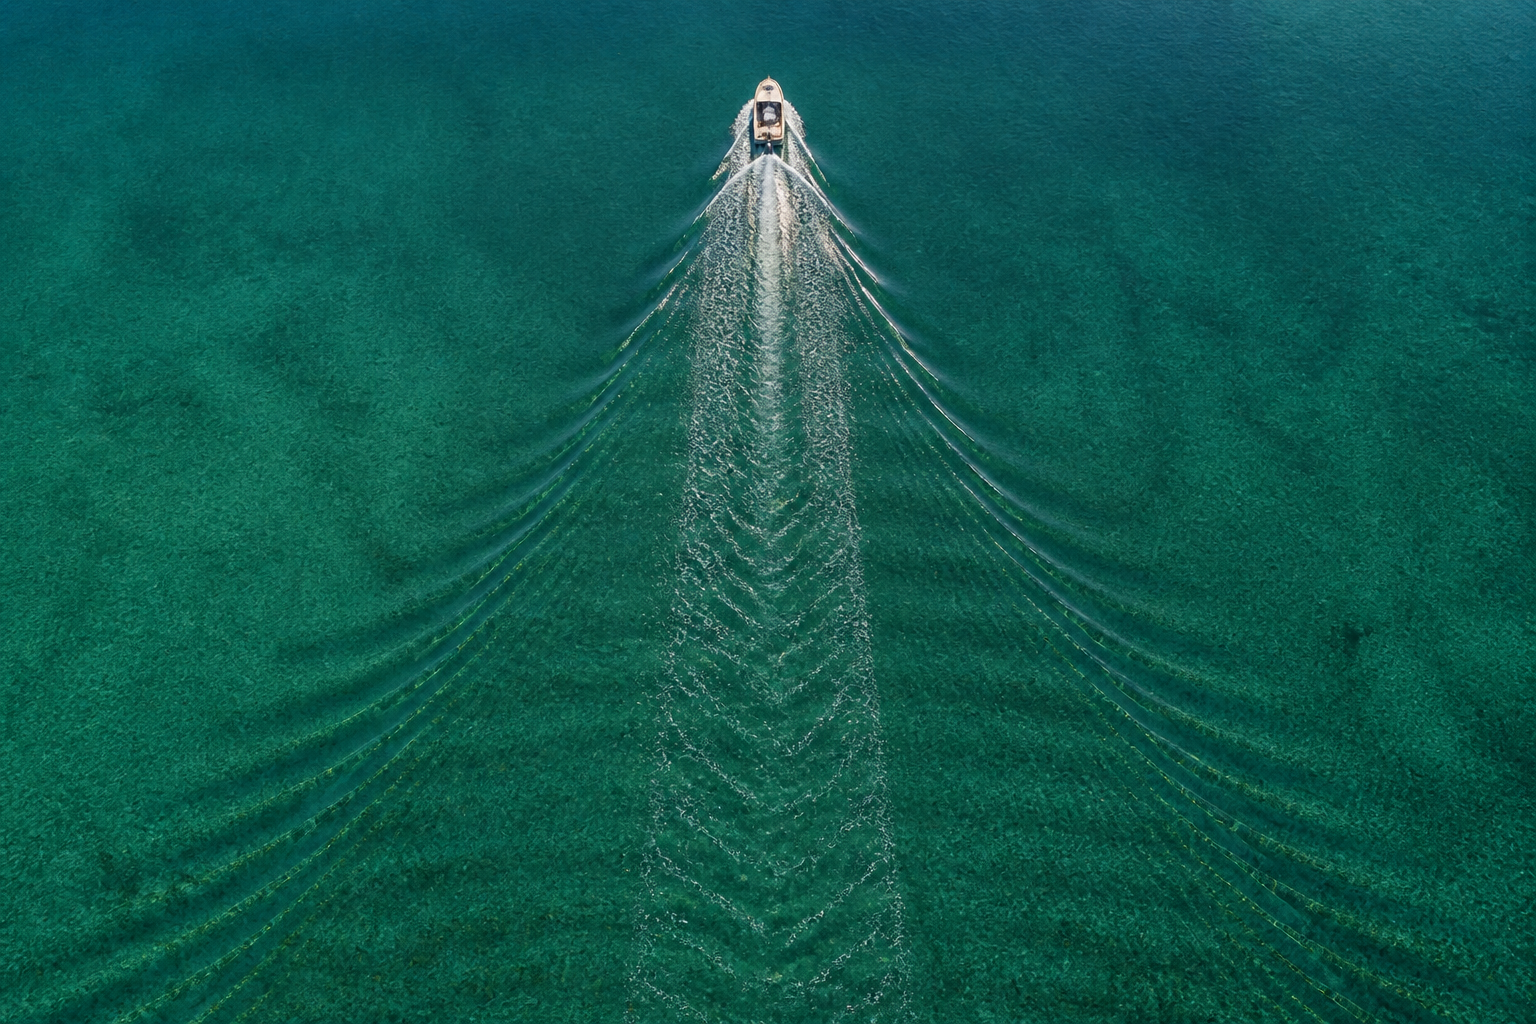
\includegraphics[width=0.56\linewidth]{images/book4/ai/b4-08-boat-wake-aerial.png}

{\small La estela de una lancha en un lago en calma: el dibujo en pluma se mantiene dentro de una cuña de ángulo fijo porque la energía de cada onda de agua viaja a la mitad de la celeridad de sus crestas --- la dispersión hecha visible.}
\end{omfigure}


\begin{example}[Klein--Gordon: más rápido que la luz, y no]\label{ex:b2:dispersion-wave-packets:superluminal}
Para $\omega^2 = \omega_c^2 + c^2k^2$: $v_\varphi = \omega/k$ y $v_g = c^2k/\omega$, luego
$v_\varphi v_g = c^2$: la \omterm{def:b2:dispersion-wave-packets:relation}{velocidad de fase} supera a $c$ (en la ionosfera, las
crestas de una onda de \qty{10}{MHz} se mueven más deprisa que la luz),
pero la \omterm{prop:b2:dispersion-wave-packets:group}{velocidad de grupo}, que es la que lleva la señal, se queda por
debajo. Una \omterm{def:b2:dispersion-wave-packets:relation}{velocidad de fase} no transporta ni energía ni información ---
las crestas son como la mancha del haz de un faro que barre una nube lejana.
\end{example}

\begin{remark}[El ensanchamiento]\label{rem:b2:dispersion-wave-packets:spreading}
Un paquete de anchura espacial $\Delta x$ contiene números de onda en un intervalo $\Delta k \sim
1/\Delta x$ (la reciprocidad de Fourier, admitida); las \omterm{prop:b2:dispersion-wave-packets:group}{velocidades de
grupo} de sus componentes difieren en $\Delta v_g \approx |\omega''|\Delta k$, de modo que al cabo de un tiempo $t$
se ha ensanchado en $|\omega''|\Delta k\,t$: duplica su anchura tras $t_{\text{ens}}
\sim \Delta x^2/|\omega''|$. Un paquete de diez ondas de aguas profundas de \qty{100}{m}
($\Delta x \approx \qty{1}{km}$, $\omega'' = -\tfrac14\sqrt{g/k^3} = \qty{-50}{m^2/s}$)
se duplica en unas seis horas; un pulso de luz de \qty{1}{ns} en una
fibra óptica se ensancha decenas de picosegundos por kilómetro --- el
límite del caudal binario de los enlaces largos. El \omterm{prop:b2:dispersion-wave-packets:group}{paquete de ondas} cuántico de
\cref{ch:b2:schrodinger-wave-functions} se ensancha por la misma razón.
\end{remark}

\section{El cable coaxial}

\begin{proposition}[Ecuaciones del telegrafista; línea sin pérdidas]\label{prop:b2:dispersion-wave-packets:coax}
\index{cable coaxial}\index{ecuaciones del telegrafista}\index{impedancia característica}\index{línea de transmisión}
Un \omterm{prop:b2:dispersion-wave-packets:coax}{cable coaxial} (o cualquier línea de dos conductores) tiene, por unidad
de longitud, una inductancia $\Lambda$ y una capacidad $\Gamma$. La tensión
$v(x, t)$ entre los conductores y la intensidad $i(x, t)$ en el conductor
interior obedecen las \emph{\omterm{prop:b2:dispersion-wave-packets:coax}{ecuaciones del telegrafista}}
\[
\frac{\partial v}{\partial x} = -\Lambda\frac{\partial i}{\partial t} , \qquad
\frac{\partial i}{\partial x} = -\Gamma\frac{\partial v}{\partial t} ,
\]
de donde la \omterm{thm:b2:waves-on-strings:equation}{ecuación de d'Alembert} para $v$ y para $i$ con
\[
c = \frac1{\sqrt{\Lambda\Gamma}} , \qquad
v = Z_c\,i \ \text{para una onda hacia } +x, \quad Z_c = \sqrt{\frac\Lambda\Gamma} ,
\]
siendo $Z_c$ la \emph{\omterm{prop:b2:dispersion-wave-packets:coax}{impedancia característica}} de la línea. Para un
\omterm{prop:b2:dispersion-wave-packets:coax}{cable coaxial} de radios $a < b$ relleno de un dieléctrico de permitividad
relativa $\varepsilon_r$, $\Lambda = \dfrac{\mu_0}{2\pi}\ln\dfrac ba$, $\Gamma =
\dfrac{2\pi\varepsilon_0\varepsilon_r}{\ln(b/a)}$, luego $c = c_0/\sqrt{\varepsilon_r}$ (unos
\qty{2e8}{m/s}, dos tercios de la velocidad de la luz) y $Z_c = \dfrac{60\,\Omega}
{\sqrt{\varepsilon_r}}\ln\dfrac ba$: \qty{50}{\ohm} o \qty{75}{\ohm} en los cables habituales.
\end{proposition}

\begin{proof}
Modélese la rodaja $[x, x + \dd x]$ como una inductancia en serie $\Lambda\dd x$ y
una capacidad en paralelo $\Gamma\dd x$: la caída de tensión a lo largo de la
rodaja vale $\Lambda\dd x\,\partial_ti$, y la corriente que se escapa por la capacidad es $\Gamma\dd x
\,\partial_tv$. Derívense cruzadamente. Para $v = f(x - ct)$, la primera ecuación
da $i = f(x - ct)/\Lambda c = v/\sqrt{\Lambda/\Gamma}$. Los valores de $\Lambda$ y de
$\Gamma$ son los del condensador cilíndrico y los de la bobina coaxial
calculados en el volumen del Año 1.
\end{proof}

\begin{omfigure}
\begin{tikzpicture}[font=\small]
  \begin{scope}
    \draw (0,0) to[L, l=$\Lambda\,\dd x$] (2.2,0) to[C, l=$\Gamma\,\dd x$] (2.2,-1.6);
    \draw (0,-1.6) -- (2.2,-1.6);
    \draw (2.2,0) -- (3.8,0); \draw (2.2,-1.6) -- (3.8,-1.6);
    \draw[->] (0.1,0.35) -- (0.7,0.35); \node[font=\footnotesize] at (0.4,0.6) {$i(x)$};
    \draw[->] (2.9,0.35) -- (3.5,0.35); \node[font=\footnotesize] at (3.2,0.6) {$i(x+\dd x)$};
    \node[font=\footnotesize] at (-0.3,-0.8) {$v(x)$}; \node[font=\footnotesize] at (4.6,-0.8) {$v(x+\dd x)$};
    \draw (-0.6,-0.2) -- (-0.6,-1.4); \draw[->] (-0.6,-1.4) -- (-0.6,-0.3);
    \node[font=\footnotesize] at (1.6,-2.3) {una rodaja de la línea};
  \end{scope}
  \begin{scope}[xshift=8.4cm, yshift=-0.8cm]
    \draw[thick, fill=omExo!30] (0,0) circle (1.3);
    \draw[thick, fill=omDef!15] (0,0) circle (1.05);
    \draw[thick, fill=omThm!40] (0,0) circle (0.3);
    \draw[<->] (0,0) -- (30:0.3) node[pos=1.6, font=\footnotesize] {$a$};
    \draw[<->] (0,0) -- (-50:1.05) node[pos=0.6, right, font=\footnotesize] {$b$};
    \node[font=\footnotesize] at (0,1.65) {dieléctrico $\varepsilon_r$, malla, alma};
    \node[font=\footnotesize] at (0,-1.75) {$Z_c = \dfrac{60\,\Omega}{\sqrt{\varepsilon_r}}\ln\dfrac ba$};
  \end{scope}
\end{tikzpicture}

{\small A la izquierda, el circuito equivalente de una rodaja $\dd x$ de
una línea sin pérdidas --- inductancia en serie, capacidad en paralelo ---
del que se siguen las \omterm{prop:b2:dispersion-wave-packets:coax}{ecuaciones del telegrafista}. A la derecha, un \omterm{prop:b2:dispersion-wave-packets:coax}{cable
coaxial} en sección; su $\Lambda$ y su $\Gamma$ dependen solo del cociente de
radios y del dieléctrico.}
\end{omfigure}

\begin{omfigure}
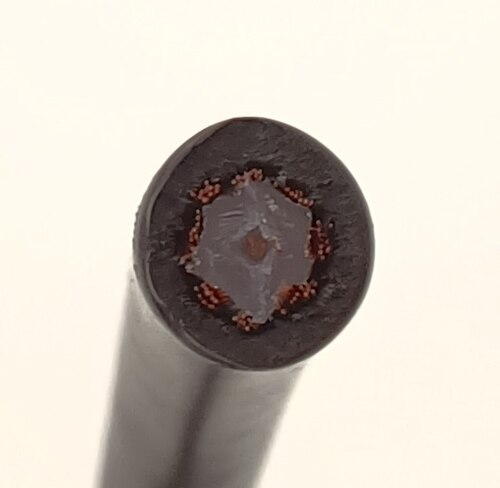
\includegraphics[width=0.46\linewidth]{images/book3/coaxial-cable.jpg}

{\small Un \omterm{prop:b2:dispersion-wave-packets:coax}{cable coaxial}: alma interior, dieléctrico y conductor exterior trenzado --- una \omterm{prop:b2:dispersion-wave-packets:coax}{línea de transmisión} cuya inductancia y cuya capacidad por metro fijan su celeridad y su \omterm{prop:b2:dispersion-wave-packets:coax}{impedancia característica}.}
\end{omfigure}

\begin{proposition}[Línea con pérdidas; la condición de no distorsión]\label{prop:b2:dispersion-wave-packets:lossy}
\index{condición de Heaviside}\index{ley de los cuadrados de Kelvin}
Con una resistencia en serie $R$ y una conductancia en paralelo $G$ por
unidad de longitud, las ecuaciones pasan a ser $\partial_xv = -\Lambda\partial_ti - Ri$, $\partial_xi =
-\Gamma\partial_tv - Gv$, y la \omterm{def:b2:dispersion-wave-packets:relation}{relación de dispersión} $\underline k^2 = (\Lambda\omega -
\iu R)(\Gamma\omega - \iu G)$: la línea es dispersiva y atenuante. Dos
límites: (i) $R/\Lambda = G/\Gamma$ (\omterm{prop:b2:dispersion-wave-packets:lossy}{condición de Heaviside}, que se alcanza
añadiendo inductancia): $\underline k = \omega\sqrt{\Lambda\Gamma} - \iu\sqrt{RG}$, toda
frecuencia viaja a la misma celeridad con la misma \omterm{def:b2:dispersion-wave-packets:complex}{atenuación} --- la línea
\emph{atenúa} pero no \emph{distorsiona}. (ii) $\Lambda \approx 0$, $G \approx 0$
(los primeros cables submarinos): $\partial_x^2v = R\Gamma\,\partial_tv$, una
ecuación de \emph{difusión} --- un pulso no se propaga, sino que se
difumina y alcanza la distancia $L$ tras un tiempo $\sim R\Gamma L^2$ (la \omterm{prop:b2:dispersion-wave-packets:lossy}{ley
de los cuadrados de Kelvin}), cien veces mayor para un cable diez veces más largo.
\end{proposition}

\begin{proof}
Sustitúyase $\eu^{\iu(\omega t - kx)}$: $-\iu kv = -(\iu\omega\Lambda + R)i$, $-\iu ki = -(\iu
\omega\Gamma + G)v$; multiplíquense. Bajo la \omterm{prop:b2:dispersion-wave-packets:lossy}{condición de Heaviside} el producto
es un cuadrado perfecto. El límite difusivo suprime los términos $\iu\omega\Lambda$ y $G$.
\end{proof}

\begin{example}[Tres cables]\label{ex:b2:dispersion-wave-packets:cables}
El cable transatlántico de 1858: un solo hilo de cobre en gutapercha,
$R \approx \qty{3}{\ohm/km}$, $\Gamma \approx \qty{0.3}{\micro F/km}$, $L = \qty{3000}{km}$:
$R\Gamma = \qty{9e-10}{s/m^2}$ y $R\Gamma L^2 \approx \qty{8}{s}$ por punto: una palabra
por minuto, y los intentos de los operadores de forzar la señal
con \qty{2}{kV} destruyeron el aislamiento en unas semanas. Una línea
telefónica cargada con bobinas cada \qty{2}{km} para cumplir la \omterm{prop:b2:dispersion-wave-packets:lossy}{condición
de Heaviside} (1900): habla nítida a lo largo de cientos de kilómetros. Un \omterm{prop:b2:dispersion-wave-packets:coax}{cable
coaxial} moderno de \qty{50}{\ohm}: $c = \qty{2e8}{m/s}$, $\Lambda = \qty{0.25}{\micro H/m}$, $\Gamma =
\qty{100}{pF/m}$, y una \omterm{def:b2:dispersion-wave-packets:complex}{atenuación}, debida al efecto pelicular en los
conductores (\cref{ch:b2:waves-in-media}), que crece como $\sqrt f$: unos
pocos \omterm{def:b2:sound-waves:decibel}{decibelios} por cada cien metros a \qty{100}{MHz}.
\end{example}

\begin{method}[Cómo leer una relación de dispersión]\label{met:b2:dispersion-wave-packets:method}
(1) Escríbase la \omterm{thm:b2:waves-on-strings:equation}{ecuación de ondas} del medio en notación compleja y
despéjese $\underline k(\omega)$. (2) Si $k$ es real: calcúlense $v_\varphi = \omega/k$
y $v_g = \dd\omega/\dd k$ (o $1/(\dd k/\dd\omega)$) y compárense: dispersivo o
no, normal ($v_g < v_\varphi$) o anómalo. (3) Si $k$ es complejo: sepárese en
propagación ($k'$) y \omterm{def:b2:dispersion-wave-packets:complex}{atenuación} ($k''$, de longitud $1/k''$); imaginario
puro significa evanescente, sin transporte. (4) Una frecuencia de corte
separa una banda propagante de otra evanescente. (5) Para una señal,
razónese sobre la envolvente a $v_g$, nunca sobre las crestas.
\end{method}

\section{Ejercicios}

\begin{exercise}[$\star$]\label{exo:b2:dispersion-wave-packets:1}
\omterm{ex:b2:dispersion-wave-packets:examples}{Ondas en aguas profundas}, $\omega^2 = gk$. (a) \omterm{def:b2:dispersion-wave-packets:relation}{Velocidad de fase}, \omterm{prop:b2:dispersion-wave-packets:group}{velocidad de
grupo} y periodo de un mar de fondo de \qty{100}{m}. (b) Un mar de fondo de
periodo \qty{14}{s}: longitud de onda, $v_\varphi$, $v_g$; tiempo que tarda su
energía en recorrer \qty{5000}{km}. (c) ¿Por qué no llega en absoluto el oleaje corto de periodo \qty{2}{s}?
\end{exercise}

\begin{exercise}[$\star$]\label{exo:b2:dispersion-wave-packets:2}
Un medio obedece $\omega^2 = \omega_c^2 + c^2k^2$ con $\omega_c = 2\pi \times \qty{1e7}{rad/s}$
y $c = \qty{3e8}{m/s}$. Para $f = \qty{20}{MHz}$: $k$, $v_\varphi$, $v_g$ y su
producto. Para $f = \qty{5}{MHz}$: $\kappa$ y la \omterm{def:b2:dispersion-wave-packets:complex}{profundidad de penetración}.
\end{exercise}

\begin{exercise}[$\star$]\label{exo:b2:dispersion-wave-packets:3}
Dos diapasones a \qty{440}{Hz} y \qty{444}{Hz}: frecuencia de batido y
periodo de las variaciones de intensidad sonora. Dos ondas de agua de
longitudes \qty{100}{m} y \qty{110}{m}: frecuencias, longitud de onda y
celeridad de la envolvente; compárese con $v_g$ a \qty{105}{m}.
\end{exercise}

\begin{exercise}[$\star$]\label{exo:b2:dispersion-wave-packets:4}
Un \omterm{prop:b2:dispersion-wave-packets:coax}{cable coaxial}: conductor interior de \qty{0.9}{mm} de diámetro y exterior
de \qty{3.0}{mm}, con polietileno ($\varepsilon_r = 2.3$). $\Lambda$, $\Gamma$, celeridad de las ondas,
\omterm{prop:b2:dispersion-wave-packets:coax}{impedancia característica} y retardo por metro; longitud de cable
equivalente a un retardo de \qty{10}{ns}. El mismo cable con aire en lugar de polietileno.
\end{exercise}

\begin{exercise}[$\star\star$]\label{exo:b2:dispersion-wave-packets:5}
\emph{La cuerda rígida.} Una cuerda de piano real obedece $\mu\partial_t^2y = T\partial_x^2y
- EI\,\partial_x^4y$ (siendo $EI$ la rigidez a flexión). (a) \omterm{def:b2:dispersion-wave-packets:relation}{Relación de dispersión} y
\omterm{def:b2:dispersion-wave-packets:relation}{velocidades de fase} y de grupo. (b) Para la cuerda la$_4$ de
\cref{ch:b2:waves-on-strings} ($T = \qty{685}{N}$, $\mu = \qty{6.1}{g/m}$, $EI =
\qty{9.8e-3}{N.m^2}$), aumento relativo de $v_\varphi$ para el octavo
armónico ($k = 8\pi/L$, $L = \qty{0.38}{m}$); compruébese con la
inarmonicidad hallada allí. (c) ¿Es la dispersión normal o anómala? ¿Qué
aspecto tiene un pulsado seco tras unas cuantas idas y vueltas?
\end{exercise}

\begin{exercise}[$\star\star$]\label{exo:b2:dispersion-wave-packets:6}
\emph{Cuerda amortiguada.} $\mu\partial_t^2y + \alpha\partial_ty = T\partial_x^2y$. (a) Dedúzcase
la \omterm{def:b2:dispersion-wave-packets:relation}{relación de dispersión}. (b) Para $\alpha \ll \mu\omega$, muéstrese que $k' \approx \omega/c$ y
$k'' \approx \alpha/2Z$; \omterm{def:b2:dispersion-wave-packets:complex}{atenuación} en \omterm{def:b2:sound-waves:decibel}{decibelios} por metro. (c) Valores: $\mu =
\qty{5}{g/m}$, $T = \qty{50}{N}$, $\alpha = \qty{0.02}{kg.m^{-1}.s^{-1}}$, $f =
\qty{100}{Hz}$: compruébese la aproximación y dese $\delta$. (d) ¿Es dispersiva
la cuerda amortiguada? ¿En qué régimen de $\alpha$ lo sería?
\end{exercise}

\begin{exercise}[$\star\star$]\label{exo:b2:dispersion-wave-packets:7}
\emph{Rizos.} Las ondas de agua cortas las gobierna la \omterm{rem:b2:viscous-flows:capillarity}{tensión superficial}: $\omega^2 =
\gamma k^3/\rho$ ($\gamma = \qty{0.072}{N/m}$); la relación completa es $\omega^2 = gk +
\gamma k^3/\rho$. (a) $v_\varphi$ y $v_g$ para ondas capilares puras; ¿cuál es
mayor? (b) Muéstrese que la \omterm{def:b2:dispersion-wave-packets:relation}{velocidad de fase} de la relación completa es
mínima en $\lambda_m = 2\pi\sqrt{\gamma/\rho g}$ y calcúlense $\lambda_m$ y $v_{\min}$.
(c) Una barca más lenta que $v_{\min}$ no deja estela: ¿por qué? (d) Las
gotas de lluvia sobre un estanque forman anillos cuyas crestas van por detrás del anillo: ¿en qué régimen?
\end{exercise}

\begin{exercise}[$\star\star$]\label{exo:b2:dispersion-wave-packets:8}
\emph{Ensanchamiento.} Un paquete de anchura inicial $\Delta x_0$ duplica su anchura
tras $t_{\text{ens}} \approx \Delta x_0^2/|\omega''(k_0)|$. (a) Un grupo de \omterm{ex:b2:dispersion-wave-packets:examples}{ondas en
aguas profundas}, $\lambda = \qty{50}{m}$, $\Delta x_0 = \qty{500}{m}$. (b) Un pulso de luz en
una fibra de vidrio: $\omega'' \approx \qty{-0.16}{m^2/s}$; un pulso de \qty{10}{ps} ($\Delta x_0 =
\qty{2}{mm}$): tiempo de ensanchamiento y distancia recorrida entretanto; lo mismo
para un pulso de \qty{1}{ns}. ¿Por qué los enlaces ópticos largos usan
pulsos más largos o fibra compensadora de dispersión?
\end{exercise}

\begin{exercise}[$\star\star$]\label{exo:b2:dispersion-wave-packets:9}
\emph{El cable submarino.} $R = \qty{3}{\ohm/km}$, $\Gamma = \qty{0.3}{\micro F/km}$,
con $\Lambda$ y $G$ despreciables. (a) Muéstrese que $v$ obedece una ecuación de difusión y
dese su difusividad. (b) \omterm{def:b2:dispersion-wave-packets:relation}{Relación de dispersión} $\underline k(\omega)$; \omterm{def:b2:dispersion-wave-packets:relation}{velocidad de
fase} y longitud de \omterm{def:b2:dispersion-wave-packets:complex}{atenuación} a \qty{1}{Hz} y a \qty{10}{Hz}. (c)
Tiempo que tarda una señal en ``llegar'' a \qty{3000}{km} ($\sim R\Gamma L^2$); palabras por
minuto. (d) El remedio de Heaviside: inductancia por kilómetro necesaria para
$R/\Lambda = G/\Gamma$ si $G = \qty{1e-7}{S/km}$; ¿por qué era difícil añadirla?
\end{exercise}

\begin{exercise}[$\star\star\star$]\label{exo:b2:dispersion-wave-packets:10}
\emph{La energía viaja a la \omterm{prop:b2:dispersion-wave-packets:group}{velocidad de grupo}.} Cuerda sobre un lecho elástico:
$\mu\partial_t^2y = T\partial_x^2y - Ky$, con la onda $y = A\cos(\omega t - kx)$ y $\omega^2 =
\omega_c^2 + c^2k^2$. (a) Densidad de energía $e = \tfrac12\mu(\partial_ty)^2 + \tfrac12T
(\partial_xy)^2 + \tfrac12Ky^2$ y flujo $\mathcal P = -T\partial_xy\,\partial_ty$: compruébese
$\partial_te + \partial_x\mathcal P = 0$. (b) Promedios temporales $\langle e\rangle$ y
$\langle\mathcal P\rangle$ para la onda. (c) Muéstrese que $\langle\mathcal P\rangle/
\langle e\rangle = c^2k/\omega = v_g$, y no $v_\varphi$. (d) ¿Qué le ocurre al
flujo de energía por debajo de la frecuencia de corte?
\end{exercise}

\begin{exercise}[$\star\star\star$]\label{exo:b2:dispersion-wave-packets:11}
\emph{Mar de fondo y tsunami.} Las ondas de agua de longitud de onda $\lambda$
sobre una profundidad $h$ obedecen $\omega^2 = gk\tanh kh$ (admitida). (a)
Recupérense los límites de aguas profundas y de aguas someras
($kh \ll 1$); celeridad de las ondas en aguas someras; ¿son dispersivas?
(b) Un tsunami de $\lambda = \qty{200}{km}$ sobre \qty{4}{km} de océano:
¿qué límite?, celeridad, periodo; tiempo para cruzar \qty{8000}{km}. (c) Su
amplitud en mar abierto es \qty{0.5}{m}: energía por unidad de longitud de cresta
(admítase $E = \tfrac12\rho gA^2$ por unidad de área) para un frente de \qty{1000}{km}; ¿qué
ocurre cuando la profundidad baja a \qty{10}{m}, si el flujo de energía $Ev_g$ se
conserva (ley de Green, $A \propto h^{-1/4}$)? (d) Un mar de fondo de \qty{100}{m}
que llega a una playa: ¿a qué profundidad empieza a sentir el fondo y por
qué giran sus crestas hasta ponerse paralelas a la orilla?
\end{exercise}

\begin{exercise}[$\star\star\star$]\label{exo:b2:dispersion-wave-packets:12}
\emph{Un pulso en una línea.} Un cable de \qty{50}{\ohm} y longitud $\ell = \qty{100}{m}$
($c = \qty{2e8}{m/s}$) se alimenta en $x = 0$ con un generador de
resistencia interna \qty{50}{\ohm} y termina en $x = \ell$ con una carga $R_L$. (a) Muéstrese
que una onda que llega al extremo se refleja con el coeficiente en
tensión $r = (R_L - Z_c)/(R_L + Z_c)$ (escríbanse $v$ e $i$ como suma de
onda incidente y reflejada e impóngase la ley de Ohm en la carga). (b) Valores para
$R_L = 50$, $0$, $\infty$, \qty{150}{\ohm}. (c) Se envía un pulso de \qty{1}{ns} y \qty{1}{V}:
qué muestra el osciloscopio situado en el generador, y cuándo, para cada
carga; por qué importan los \qty{50}{\ohm} del generador. (d) Un fallo en un cable
enterrado devuelve un eco al cabo de \qty{1.8}{\micro s}: ¿dónde está? (Reflectometría
en el dominio del tiempo.)
\end{exercise}

\section{Problema: el cable y el mar}

\begin{problem}[{Problema de fin de semana --- la dispersión en acción: el
cable telegráfico que difuminaba los puntos, el mar de fondo que anuncia
una tormenta, el tsunami que cruza un océano y el paquete que se ensancha}]
\label{pb:b2:dispersion-wave-packets:1}

\medskip
\noindent\textbf{Parte I --- El cable telegráfico.}
El cable transatlántico de 1866: $R = \qty{2.0}{\ohm/km}$, $\Gamma = \qty{0.25}{\micro F/km}$,
$\Lambda = \qty{0.5}{mH/km}$, $G$ despreciable, longitud $L = \qty{3500}{km}$.
\begin{enumerate}
  \item Escríbanse las \omterm{prop:b2:dispersion-wave-packets:coax}{ecuaciones del telegrafista} con $R$ y dedúzcase la
        \omterm{def:b2:dispersion-wave-packets:relation}{relación de dispersión} $\underline k^2 = \Gamma\omega(\Lambda\omega - \iu R)$.
  \item ¿A qué frecuencia iguala $\Lambda\omega$ a $R$? Conclúyase que a las
        frecuencias telegráficas (unos pocos hercios) la línea está en
        régimen difusivo.
  \item En ese régimen, $\underline k = \sqrt{-\iu R\Gamma\omega}$: dense $k'$ y $k''$
        (recuérdese que $\sqrt{-\iu} = (1 - \iu)/\sqrt2$); \omterm{def:b2:dispersion-wave-packets:relation}{velocidad de fase}
        y longitud de \omterm{def:b2:dispersion-wave-packets:complex}{atenuación} a \qty{1}{Hz} y a \qty{4}{Hz}.
  \item \omterm{def:b2:dispersion-wave-packets:complex}{Atenuación} en \omterm{def:b2:sound-waves:decibel}{decibelios} a lo largo de todo el cable a \qty{1}{Hz}
        y a \qty{4}{Hz}. ¿Qué frecuencia sobrevive? ¿Qué le hace eso a un
        punto seco?
  \item Estimación de Kelvin del tiempo de tránsito, $R\Gamma L^2$; ritmo
        práctico del cable en palabras por minuto si una palabra son unos
        $10$ puntos y rayas y los puntos no deben solaparse.
  \item Heaviside propuso subir $\Lambda$: ¿qué valor hace $\Lambda\omega = R$
        a \qty{4}{Hz}, y cuáles serían entonces la celeridad y la
        \omterm{def:b2:dispersion-wave-packets:complex}{atenuación} (tómese $G = 0$, de modo que la condición
        $R/\Lambda = G/\Gamma$ no puede cumplirse exactamente: úsese la
        relación general a esa frecuencia)?
  \item Una fibra óptica moderna transporta \qty{1e10}{bit/s}: compárese
        con la pregunta 5, en potencias de diez.
\end{enumerate}

\medskip
\noindent\textbf{Parte II --- El mar de fondo.}
Aguas profundas: $\omega^2 = gk$.
\begin{enumerate}[resume]
  \item \omterm{def:b2:dispersion-wave-packets:relation}{Velocidades de fase} y de grupo en función del periodo $T$.
  \item Una tormenta a \qty{4000}{km} de una costa genera olas de periodos
        entre \qty{6}{s} y \qty{18}{s}: instante de llegada de cada
        extremo; duración del episodio de mar de fondo.
  \item Muéstrese que en una costa situada a la distancia $D$ el periodo
        que llega cumple $1/T = gt/4\pi D$, contando $t$ desde la
        tormenta: $1/T$ crece linealmente con el tiempo. Una boya registra
        $T = \qty{16}{s}$ un día a mediodía y $T = \qty{12}{s}$ exactamente
        \qty{24}{h} después: distancia de la tormenta.
  \item La energía por unidad de área de un mar de fondo de amplitud $A$ vale $\tfrac12\rho
        gA^2$; potencia que atraviesa una línea de \qty{1}{m} de cresta, para $A =
        \qty{1.5}{m}$ y $T = \qty{12}{s}$. (Úsese la \omterm{prop:b2:dispersion-wave-packets:group}{velocidad de grupo}: ¿por qué?)
  \item Un parque undimotriz de \qty{1}{km} de frente con un rendimiento del $30\%$:
        potencia eléctrica; compárese con un aerogenerador (\qty{3}{MW}).
  \item Una barca a \qty{5}{m/s} en aguas profundas deja tras de sí una
        estela estacionaria: ¿qué longitud de onda tiene una \omterm{def:b2:dispersion-wave-packets:relation}{velocidad de
        fase} igual a la celeridad de la barca y la sigue por tanto? ¿Por
        qué el dibujo se arrastra en forma de V, más estrecha de lo que
        sugeriría la propia apertura de las crestas (piénsese en $v_g = v_\varphi/2$)?
  \item Observando un grupo de mar de fondo desde un acantilado,
        descríbase qué hace una cresta concreta mientras el grupo pasa
        por una boya fija; cuántas crestas contiene un grupo de duración
        \qty{2}{min} con $T = \qty{12}{s}$, y a cuántas ``vidas'' de
        cresta corresponde eso.
\end{enumerate}

\medskip
\noindent\textbf{Parte III --- El tsunami.}
$\omega^2 = gk\tanh kh$; profundidad del Pacífico $h = \qty{4.0}{km}$.
\begin{enumerate}[resume]
  \item Un terremoto levanta \qty{2}{m} una zona del fondo marino de
        \qty{100}{km}; la onda tiene $\lambda \approx \qty{200}{km}$: compruébese
        que es una onda de aguas someras y dense su celeridad, su periodo
        y el tiempo que tarda en llegar a una costa situada a \qty{6000}{km}.
  \item ¿Es dispersiva? Compárese con el mar de fondo de la parte II:
        ¿llega antes o después de lo que llegaría este? ¿Cuál llega como
        un único pulso?
  \item Su altura en mar abierto es \qty{0.6}{m}: energía por metro
        cuadrado; energía total de un frente de \qty{500}{km} de largo
        repartida sobre una longitud de onda; compárese con una explosión
        de \qty{1}{Mt} (\qty{4.2e15}{J}).
  \item Ley de Green: altura cuando la profundidad baja a \qty{20}{m} cerca
        de la orilla (con el flujo de energía $\tfrac12\rho gA^2v_g$ conservado y $v_g = \sqrt{gh}$);
        celeridad y longitud de onda allí; por qué la onda se empina
        entonces y rompe como un muro.
  \item Un barco en alta mar no nota el paso del tsunami: ¿por qué?
  \item Dos mareógrafos separados \qty{6000}{km} registran la onda: qué da
        el tiempo de viaje y por qué la celeridad medida es algo menor
        que $\sqrt{gh}$ sobre un océano de profundidad variable.
\end{enumerate}

\medskip
\noindent\textbf{Parte IV --- El paquete que se ensancha.}
\begin{enumerate}[resume]
  \item Para aguas profundas, calcúlese $\omega''(k) = \dd^2\omega/\dd k^2$ y su
        valor para $\lambda = \qty{100}{m}$.
  \item Se suelta un paquete de \qty{10}{} de esas ondas ($\Delta x_0 \approx \qty{1}{km}$):
        tiempo de ensanchamiento $\Delta x_0^2/|\omega''|$; distancia recorrida
        entretanto por el paquete.
  \item Explíquese con palabras por qué un paquete de espectro más
        estrecho (un tren más largo) se ensancha más despacio, y por qué
        el tsunami de la parte III apenas se ensancha.
  \item La misma estimación para un electrón de longitud de onda
        \qty{0.1}{nm} localizado en \qty{1}{nm}, con $\omega = \hbar k^2/2m$ ($\hbar =
        \qty{1.05e-34}{J.s}$, $m = \qty{9.1e-31}{kg}$): tiempo de
        ensanchamiento y distancia recorrida --- el primer contacto con el
        \omterm{prop:b2:dispersion-wave-packets:group}{paquete de ondas} cuántico de \cref{ch:b2:schrodinger-wave-functions}.
  \item Resúmase en una tabla: para el cable, el mar de fondo, el tsunami
        y el electrón, la \omterm{def:b2:dispersion-wave-packets:relation}{relación de dispersión}, $v_\varphi$, $v_g$ y si el
        medio ensancha o solo atenúa.
\end{enumerate}
\end{problem}
